\documentclass[11pt]{article}

\usepackage[a4paper, total={6in, 8in}]{geometry}
\usepackage{graphicx}
\usepackage{multirow,multicol}
\usepackage{enumitem}
\usepackage{subcaption}
\usepackage{multirow,multicol}
% set spacing in tables

\graphicspath{ {./Img/} }
\title{July2023 CSE300 Week9 Online Evaluation}
\author{2005020}
\date{\today}
\graphicspath{ {./Images/} }

\begin{document}

%style 1 npr 
\noindent $^nP_r$ $^nC_r$

$( ^n_r ) $ 


\noindent Some text 
this got indented 
 this did not :)

 $\gamma$ $\cap$ $\bigcap$ $\cup$ $\bigcup$

 \textit{THis is italic \emph{This is normal :)} This is again italic}

% rendering image at top of current page
 \begin{figure}[t]
     \centering
     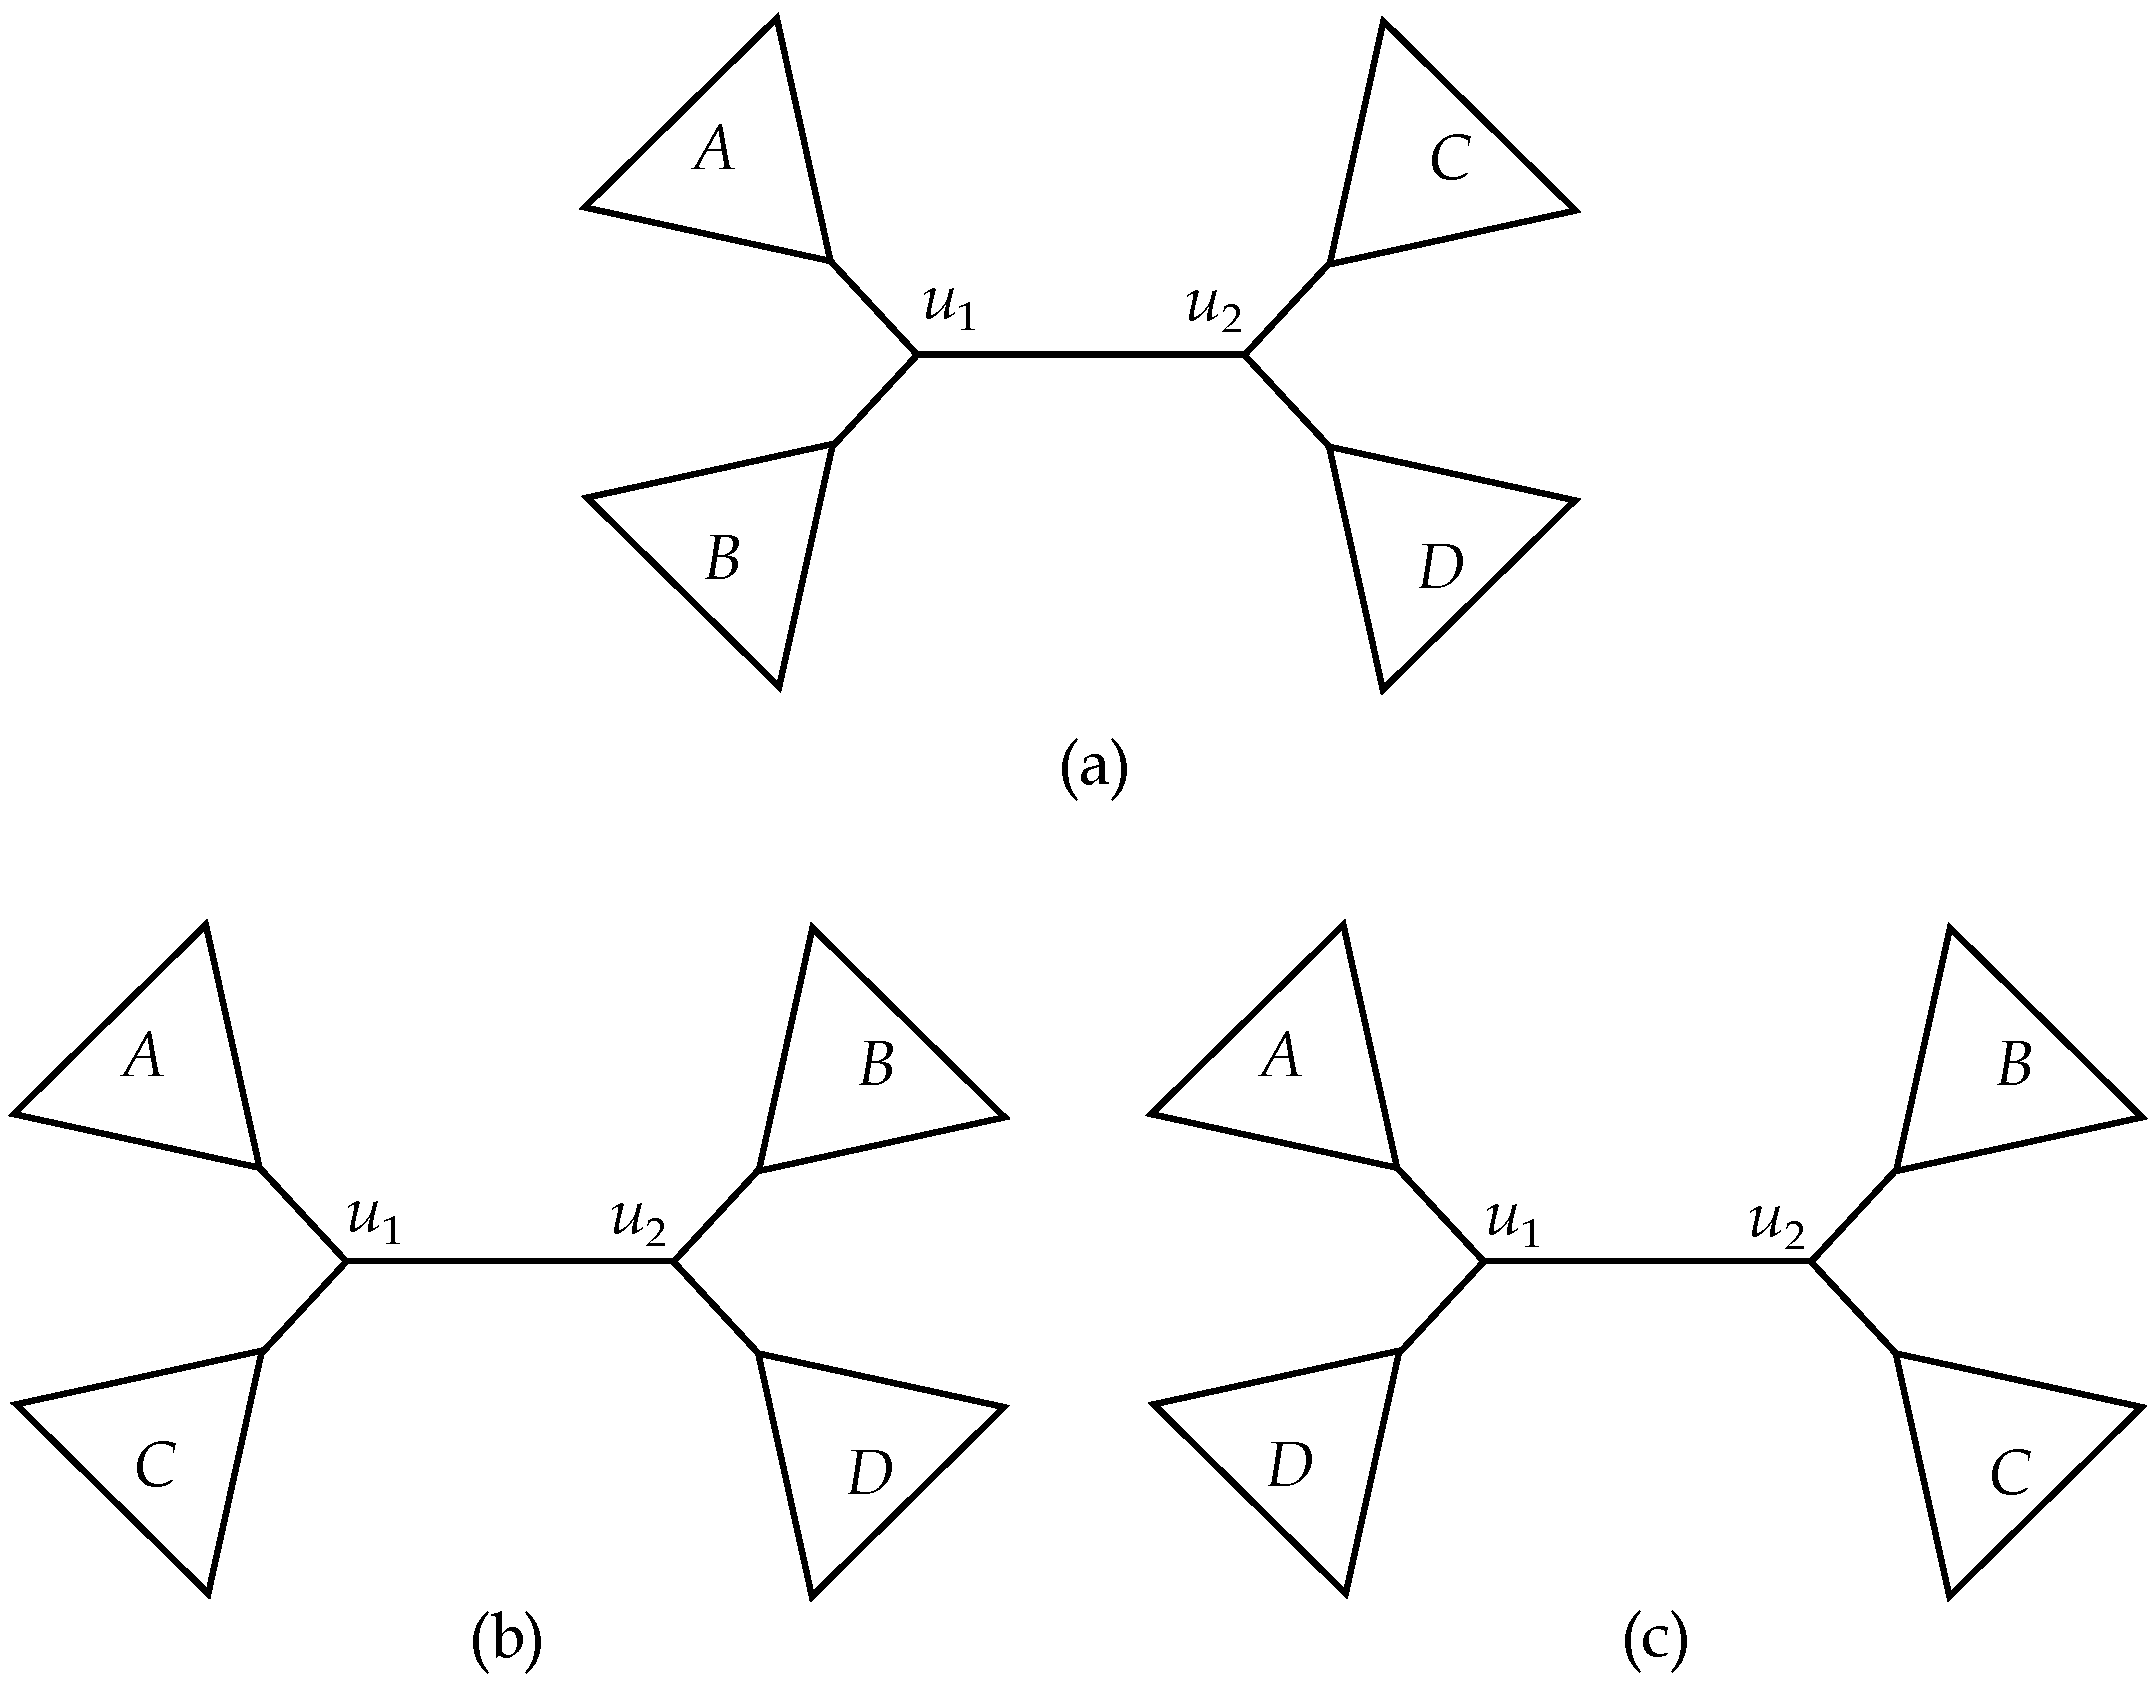
\includegraphics[width = 0.3\textwidth]{Img/Practice_Problem_4.pdf}
     \caption{Caption}
     \label{fig:enter-label}
 \end{figure}

 %rendering image at bottom of current page
 \begin{figure}[b]
     \centering
     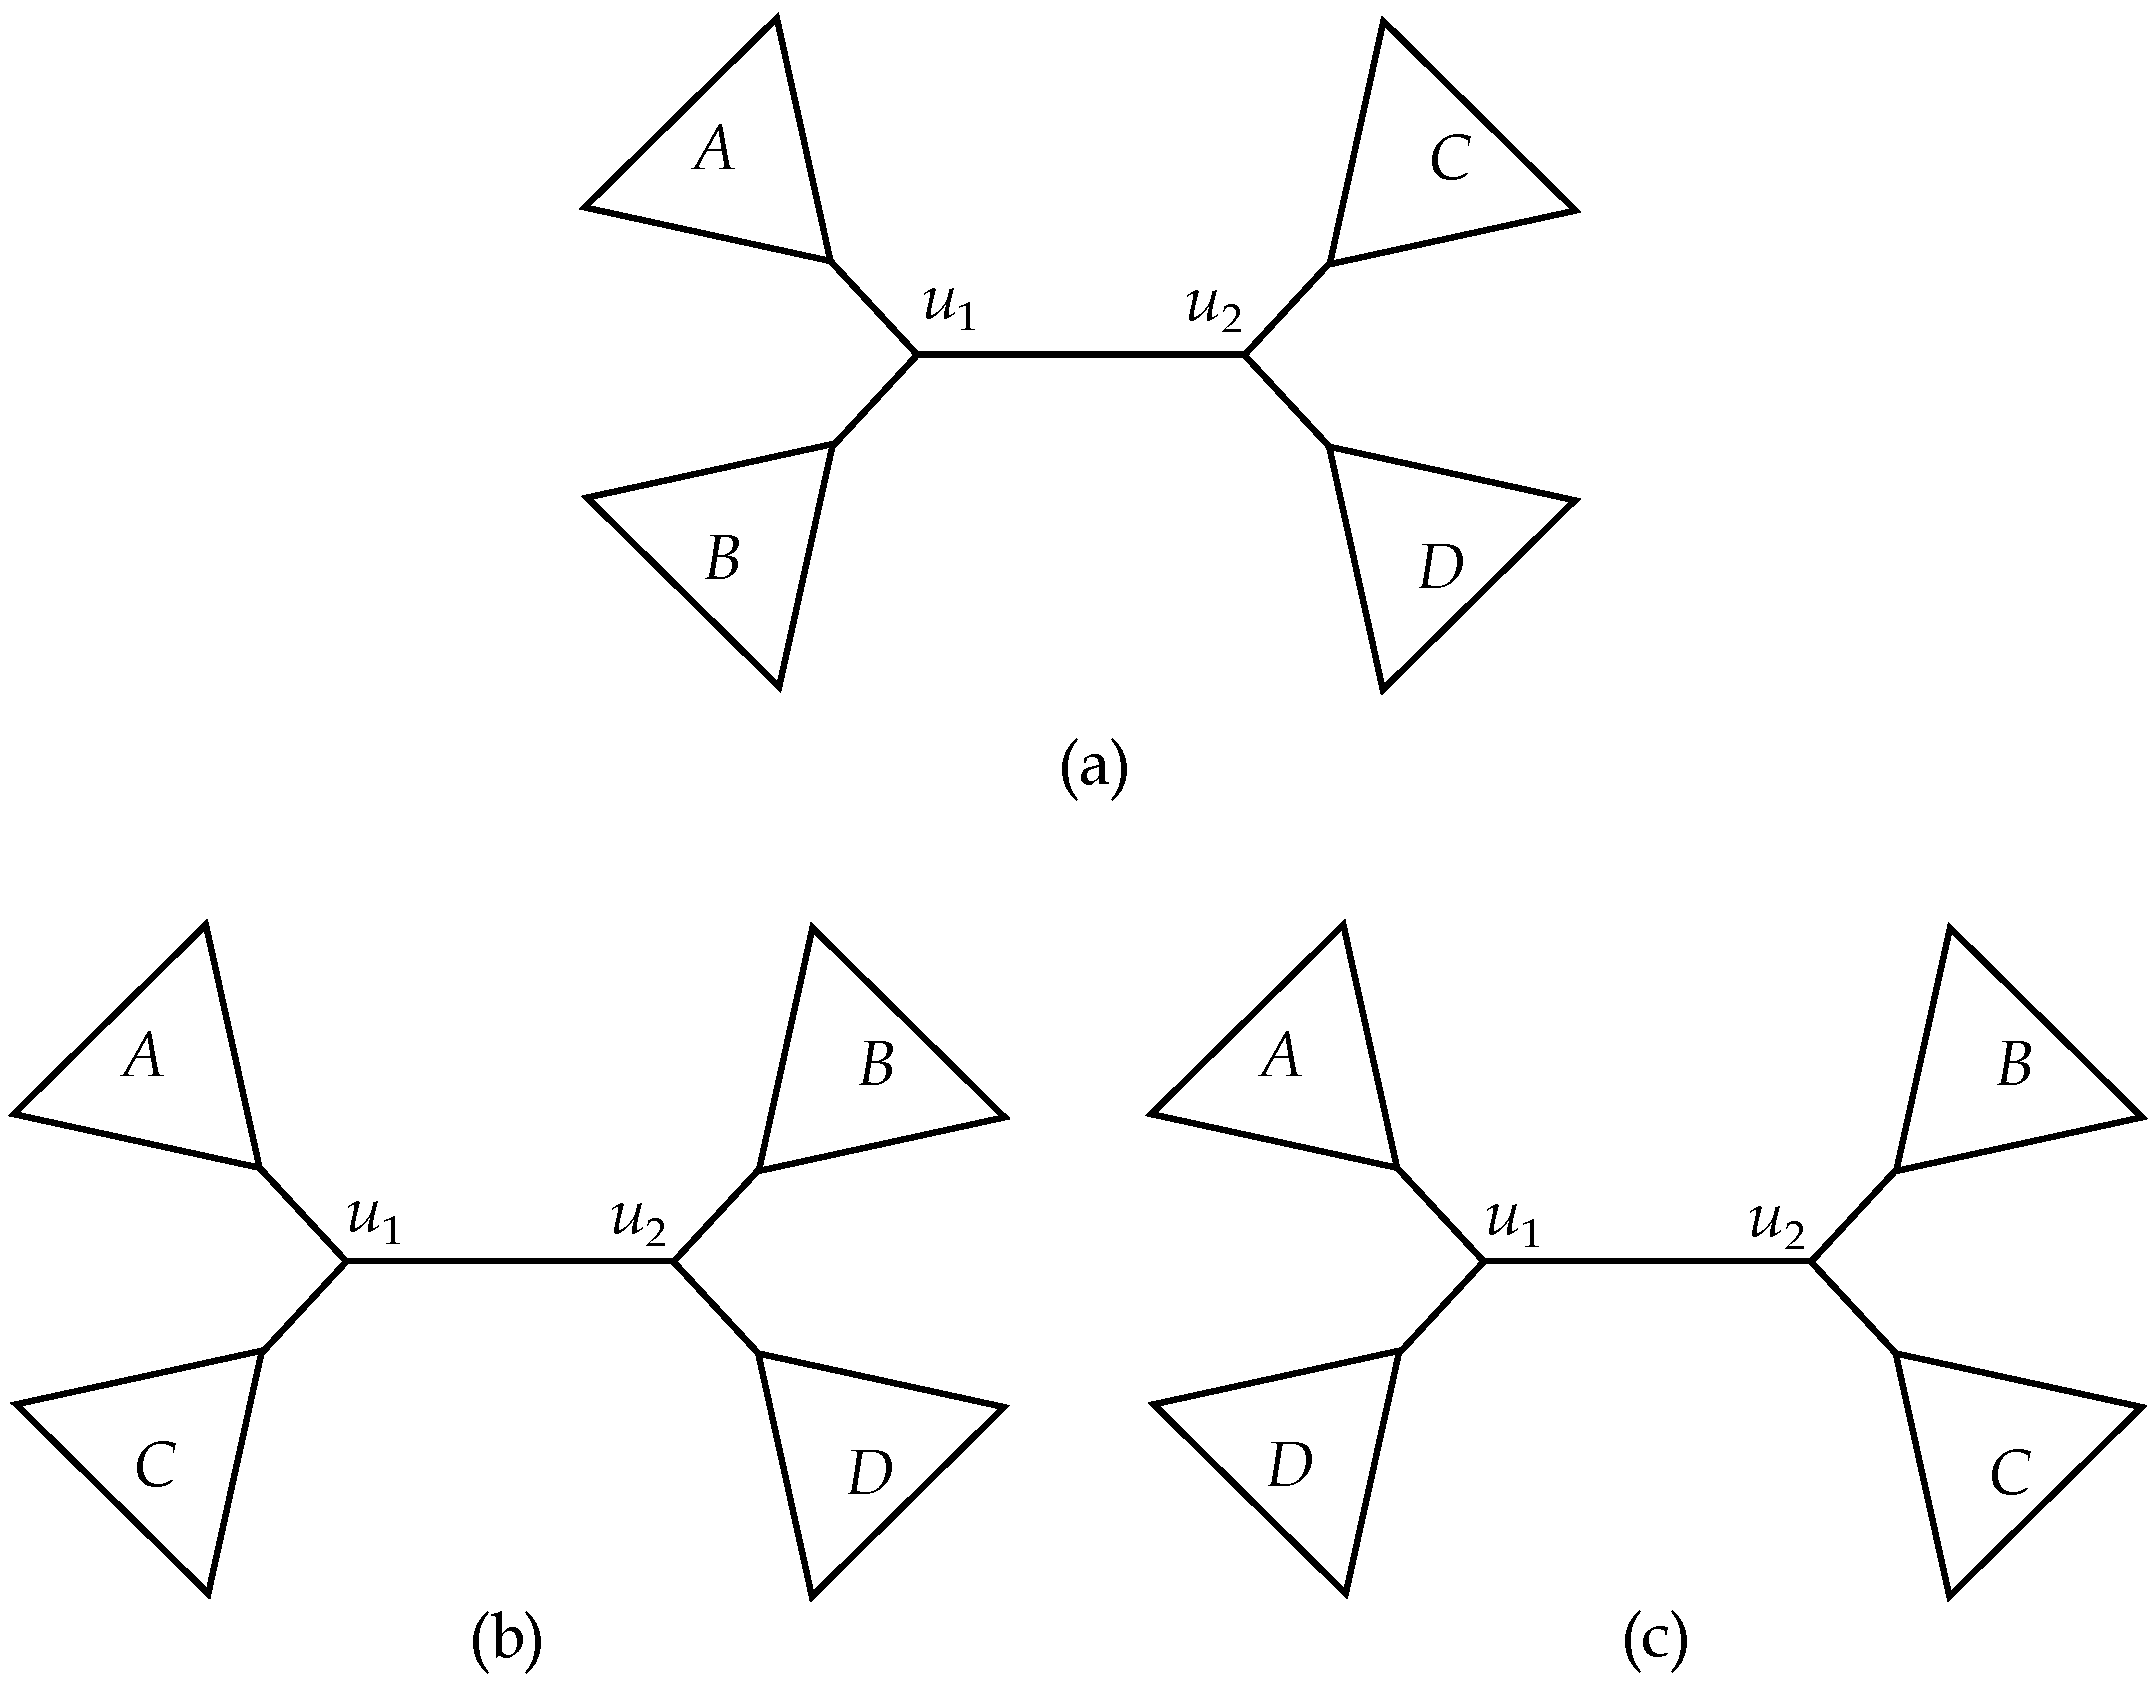
\includegraphics[width = 0.3\textwidth]{Img/Practice_Problem_4.pdf}
     \caption{Caption}
     \label{fig:enter-label}
 \end{figure}

 %using subfigure
\begin{figure}
\centering
\begin{subfigure}{.5\textwidth}
  \centering
  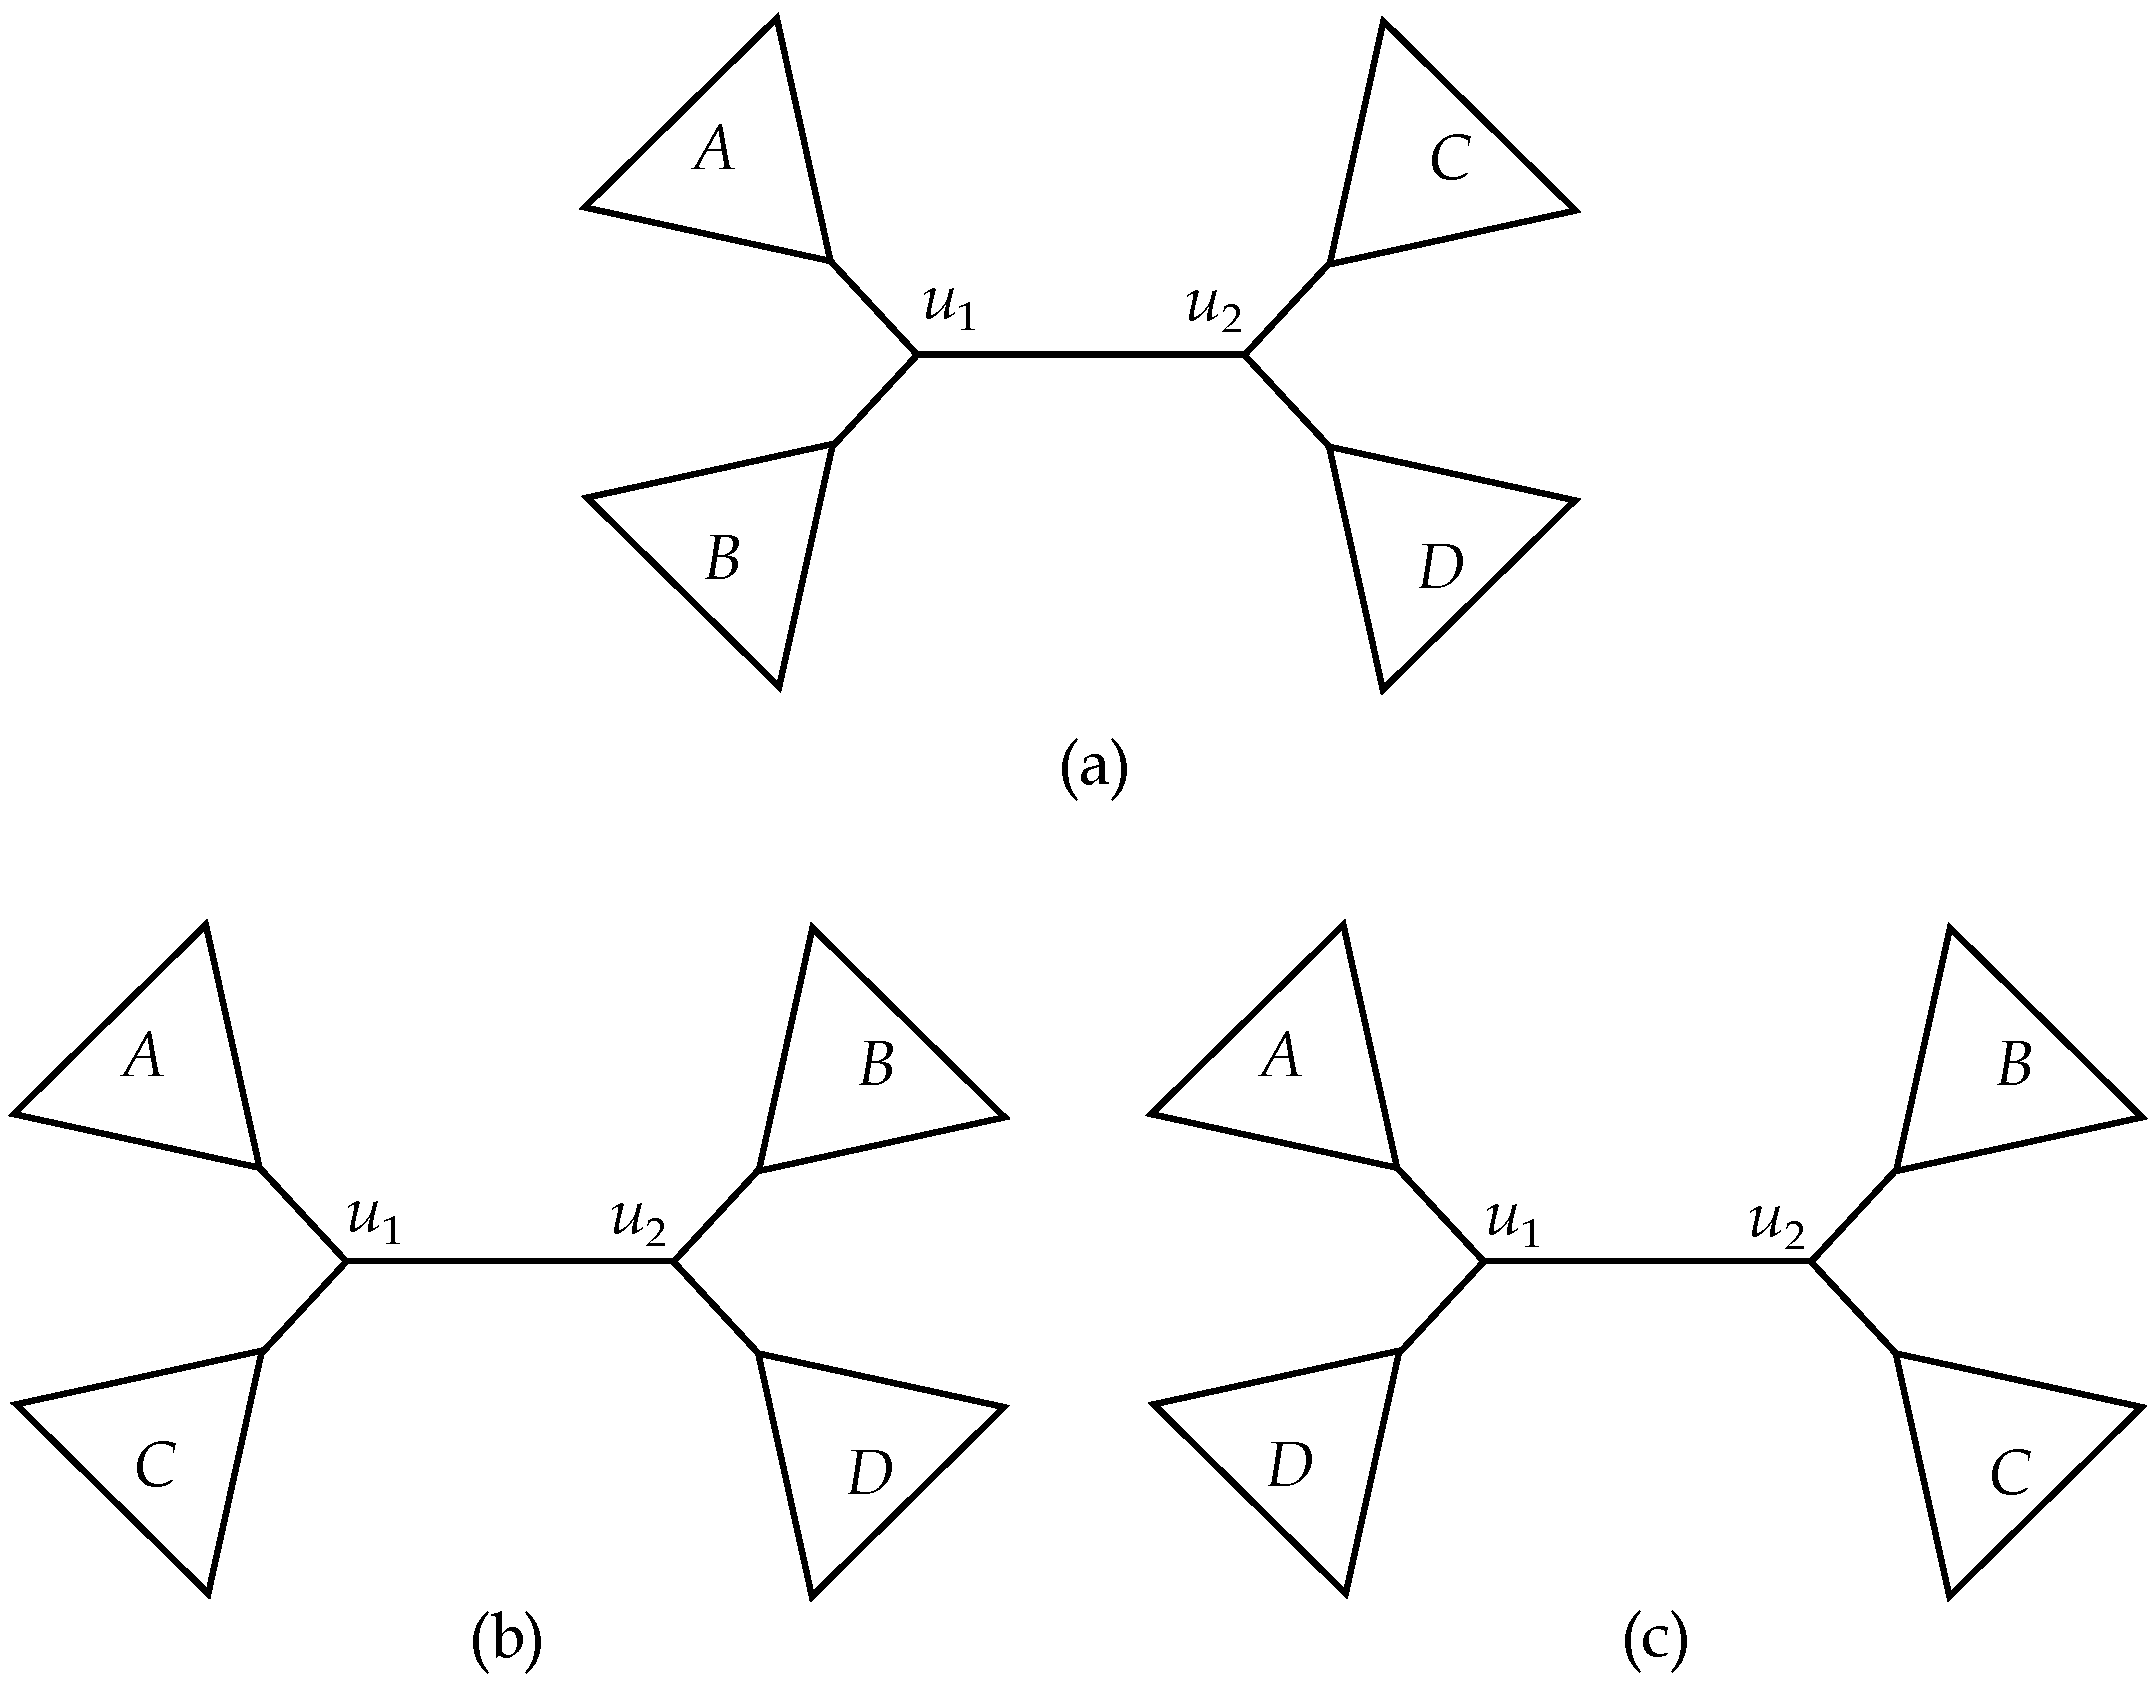
\includegraphics[angle=90,width=.4\linewidth]{Img/Practice_Problem_4.pdf}
  \caption{}
  \label{fig:sub1}
\end{subfigure}%
\begin{subfigure}{.5\textwidth}
  \centering
  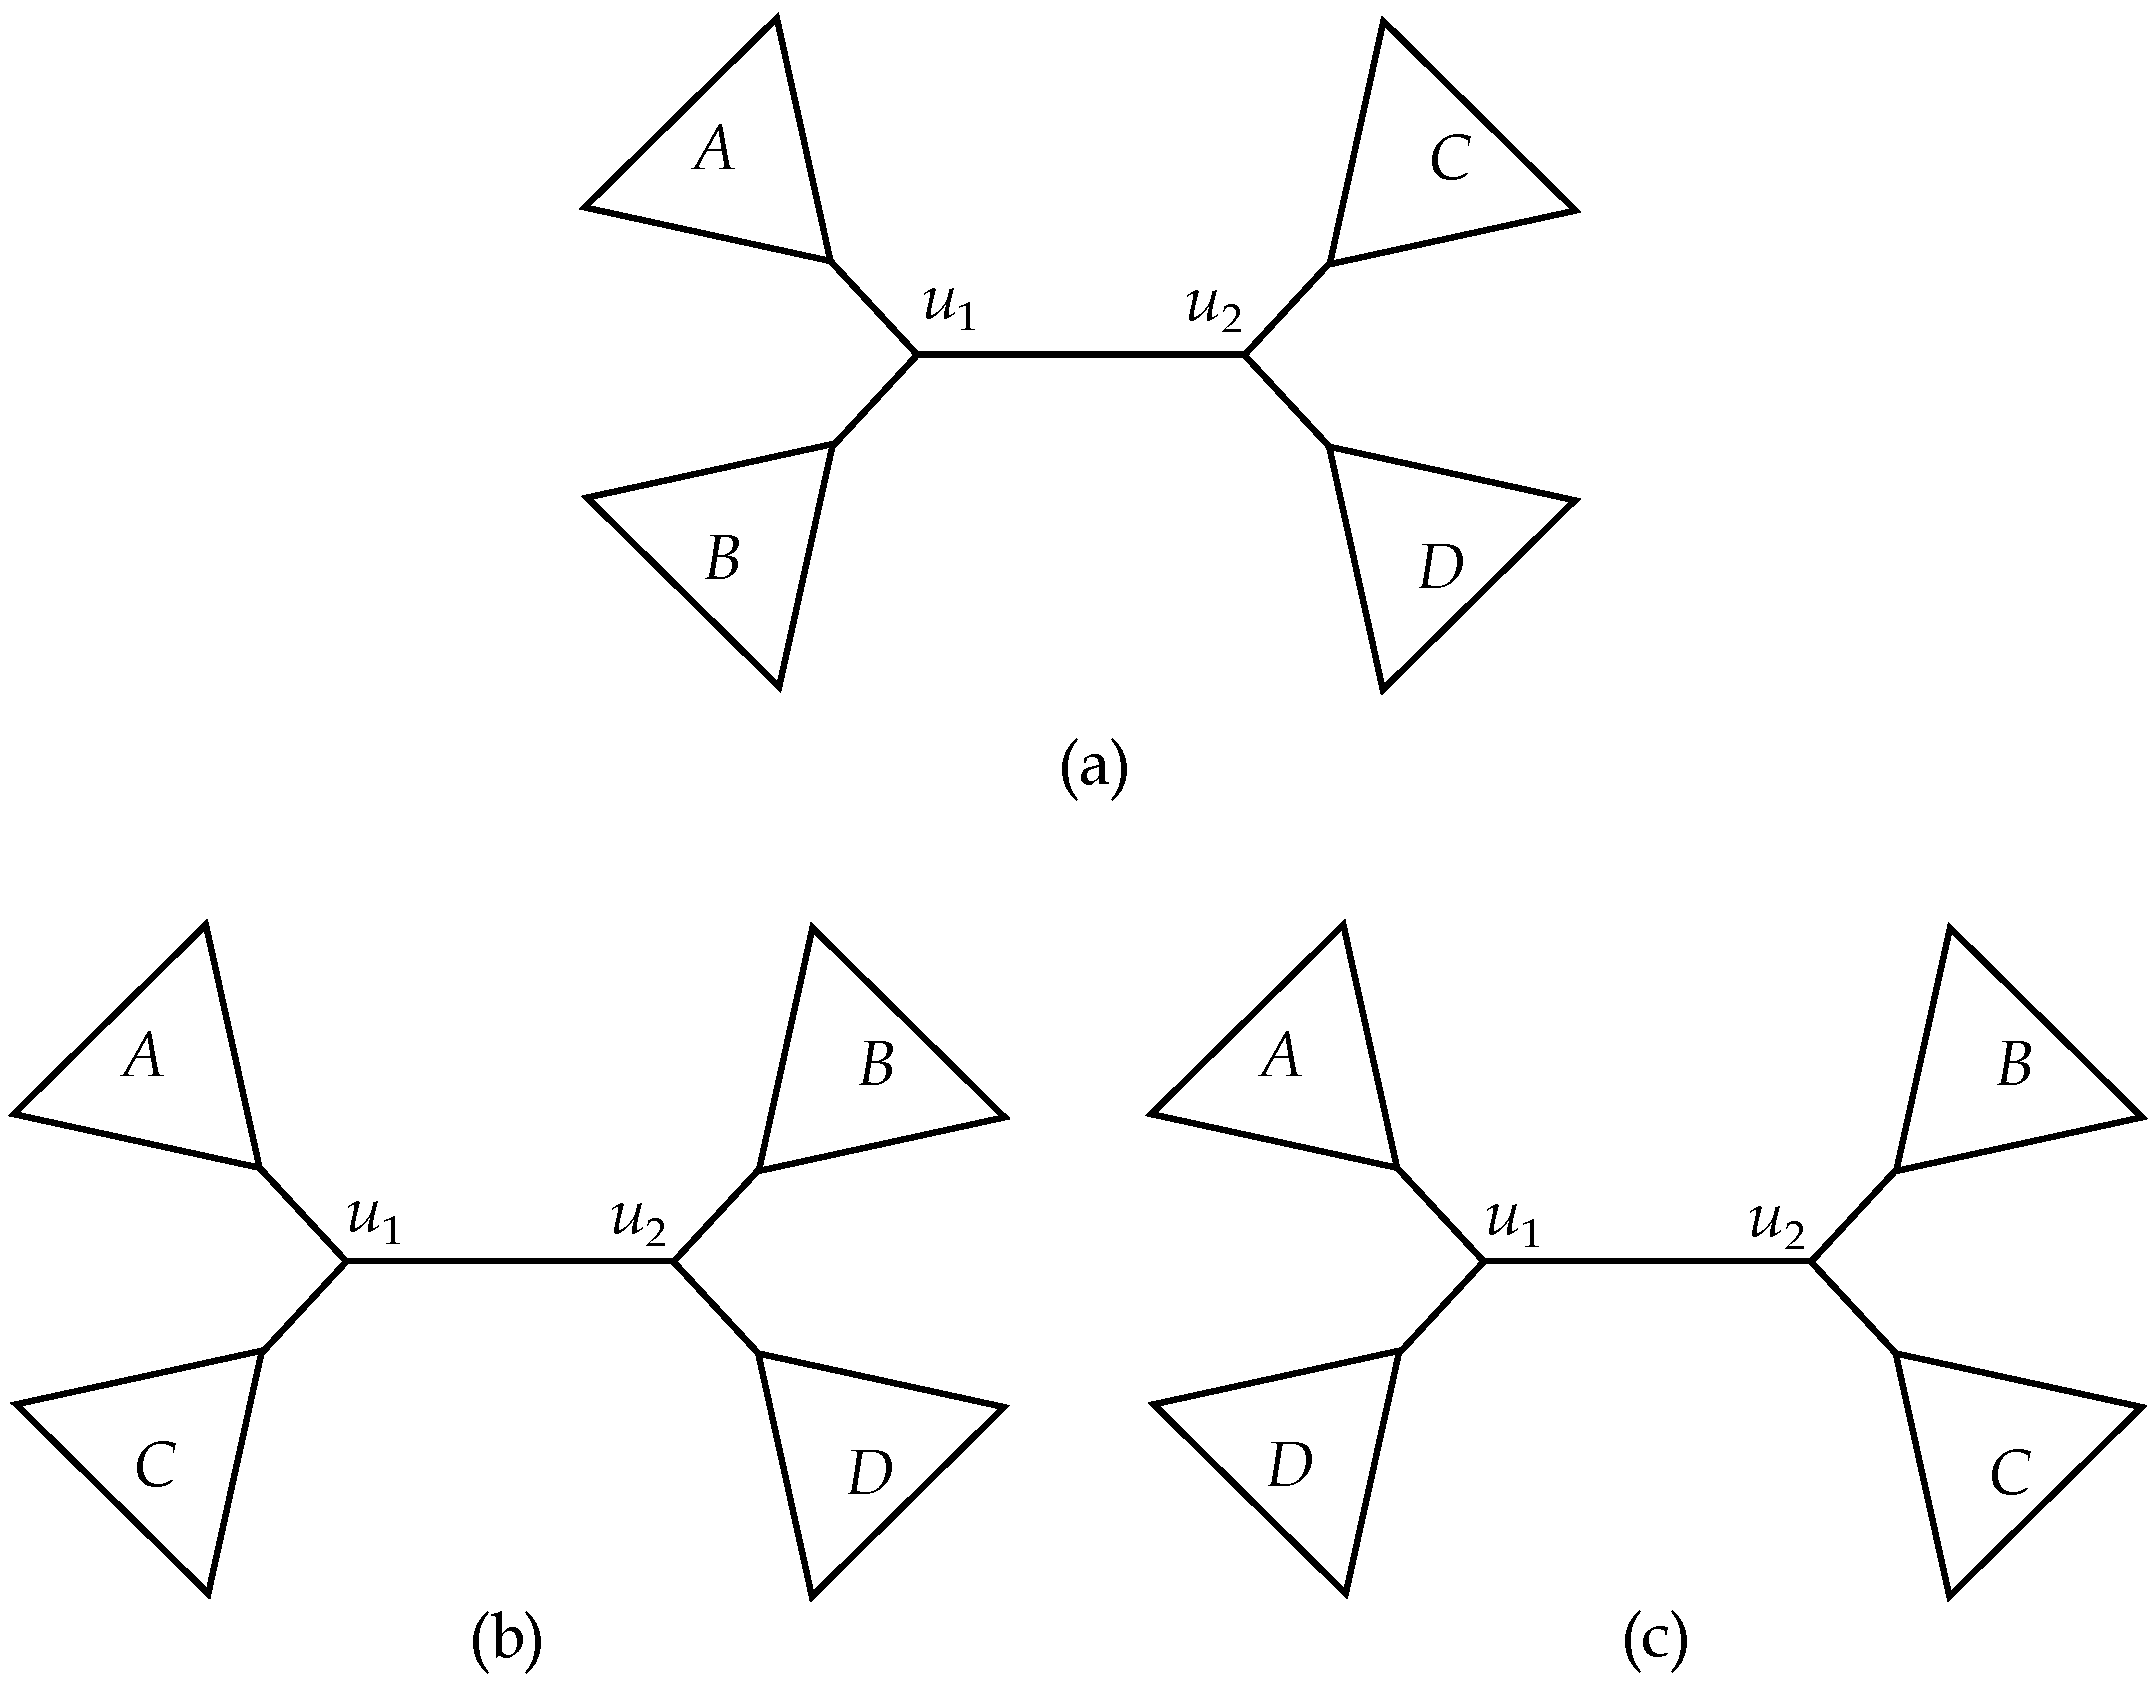
\includegraphics[angle=-90,width=.4\textwidth]{Img/Practice_Problem_4.pdf}
  \caption{}
  \label{fig:sub2}
\end{subfigure}
\caption{A figure with two subfigures}
\label{fig:test}
\end{figure}
 
\end{document}